% LaTeX source for PyMS User Guide

\documentclass[twoside,a4paper]{book}

\usepackage{epsfig}
\usepackage{graphicx}
\usepackage{makeidx}
\usepackage{tlk2e/tlk2e}
\usepackage{url}

\setlength{\topmargin}{0.0cm}
\setlength{\evensidemargin}{0.0cm}
\setlength{\oddsidemargin}{0.0cm}
\setlength{\textwidth}{16.0cm}
\setlength{\textheight}{23.0cm}
%\setlength{\footskip}{0.0cm}

\parskip 0.2cm
\parindent 0cm
\makeindex

\begin{document}

\frontmatter

\title{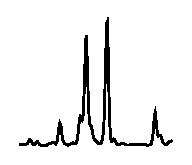
\includegraphics{logo/PyMS.eps}
\Large{PyMS User Guide}}
\author{Andrew Isaac and Vladimir Liki\'{c}\\
with contributions from:\\
\medskip}

\medskip

\version{PyMS version 1.0}

\abstract{A Python toolkit for processing of chromatography--mass spectrometry
data}

\maketitle
\tableofcontents

\input epsf

\newpage

\setcounter{chapter}{1}
\setcounter{section}{0}
\pagenumbering{arabic}
% chapter01.tex

 %%%%%%%%%%%%%%%%%%%%%%%%%%%%%%%%%%%%%%%%%%%%%%%%%%%%%%%%%%%%%%%%%%%%%%%%%%%%%
 %                                                                           %
 %    PyMS documentation                                                     %
 %    Copyright (C) 2005-8 Vladimir Likic                                    %
 %                                                                           %
 %    The files in this directory provided under the Creative Commons        %
 %    Attribution-NonCommercial-NoDerivs 2.1 Australia license               %
 %    http://creativecommons.org/licenses/by-nc-nd/2.1/au/                   %
 %    See the file license.txt                                               %
 %                                                                           %
 %%%%%%%%%%%%%%%%%%%%%%%%%%%%%%%%%%%%%%%%%%%%%%%%%%%%%%%%%%%%%%%%%%%%%%%%%%%%%

\chapter{Introduction}

\section{About PyMS}

PyMS is a Python toolkit for processing of chromatography--mass spectrometry
data. The main idea behind PyMS is to provide a framework and a set of
components for rapid development and testing of methods for processing of
chromatography--mass spectrometry data. An important objective of PyMS is
to decouple processing methods form visualization and the concept of
interactive processing. This is useful for high-throughput processing tasks
and when there is a need to run calculations in the batch mode.

PyMS is modular and consists of several sub-packages written in Python
programming language \cite{python}. PyMS is released as open source,
under the GNU Public License version 2.

There are four parts of the pyms project:

\begin{itemize}
  \item pyms -- The PyMS code
  \item pyms-docs -- The PyMS documentation
  \item pyms-test -- Examples of PyMS use
\end{itemize}

Each part is a separate project on Google Code that can be downloaded
separately. The data used in PyMS documentation and examples is available
from the Bio21 Institute server:\\
{\tt http://bioinformatics.bio21.unimelb.edu.au/pyms-data/}\\
In addition, the current PyMS API documentation is available from here:\\
{\tt http://bioinformatics.bio21.unimelb.edu.au/pyms.api/index.html}

\section{PyMS installation}

There are several ways to install PyMS depending your computer configuration
and preferences. The recommended way install PyMS is to compile Python
from sources and install PyMS within the local Python installation. This
procedure is described below.

PyMS has been developed on Linux, and a detailed installation instructions
for Linux are given below. Installation on any Unix-like system should be
similar. We have not tested PyMS under Microsoft Windows.

\subsection{Downloading PyMS source code}

PyMS source code resides on Google Code servers, and can be accessed
from the following URL: http://code.google.com/p/pyms/. Under the
section "Source" one can find the instructions for downloading the
source code. The same page provides the link under "This project's
Subversion repository can be viewed in your web browser" which allows
one to browse the source code on the server without actually downloading
it.

Google Code maintains the source code with the program `subversion'
(an open-source version control system). To download the source code
one needs to use the subversion client program called `svn'. The `svn'
client exists for all mainstream operating systems\footnote{For example,
on Linux CentOS 4 we have installed the RPM package
`subversion-1.3.2-1.rhel4.i386.rpm' to provide us with the subversion
client `svn'.}, for more information see http://subversion.tigris.org/.
The book about subversion is freely available on-line at
http://svnbook.red-bean.com/. Subversion has extensive functionality.
However only the very basic functionality is needed to download PyMS
source code.

If the computer is connected to the internet and the subversion client
is installed, the following command will download the latest PyMS source
code:

\begin{verbatim}
$ svn checkout http://pyms.googlecode.com/svn/trunk/ pyms
A    pyms/Peak
A    pyms/Peak/__init__.py
A    pyms/Peak/List
A    pyms/Peak/List/__init__.py
.....
Checked out revision 71.
\end{verbatim}

\subsection{PyMS installation}

PyMS installation consists of placing the PyMS code directory (pyms/) in
place visible to Python interpreter.  This can be in the standard place
for 3rd party software (the directory site-packages/). If PyMS code is
placed in a non-standard place the Python interpreter needs to be made
aware of it before before it is possible to import PyMS modules (see the
Python sys.path.append() command).

We recommend compiling your own Python installation for PyMS.

In addition to the PyMS core source code, a number of external packages
is used to provide additional functionality. These are explained below.

\subsection{\label{subsec:numpy}Package `NumPy'}

The package NumPy is provides numerical capabilities to Python. This
package is used throughout PyMS (and also required for some external
packages used in PyMS), to its installation is mandatory.

The NumPy web site {\tt http://numpy.scipy.org/} provides the installation
instructions and the link to the source code.

\subsection{\label{subsec:pycdf}Package `pycdf' (required for reading
ANDI-MS files)}

The pycdf (a python interface to Unidata netCDF library) source and
installation instructions can be downloaded from\\
{\tt http://pysclint.sourceforge.net/pycdf/}. Follow the installation
instructions to install pycdf.

\subsection{\label{subsec:pycluster}Package `Pycluster' (required for peak
alignment by dynamic programming)}

The peak alignment by dynamic programming is located in the subpackage
pyms.Peak.List.DPA. This subpackage used the Python package `Pycluster'
as the clustering engine. Pycluster with its installation instructions
can be found here:\\
{\tt http://bonsai.ims.u-tokyo.ac.jp/~mdehoon/software/cluster/index.html}.

\subsection{\label{subsec:scipy-ndmage}Package `scipy.ndimage' (required
for TopHat baseline corrector)}

If the full SciPy package is installed the `ndimage' will be available. However
the SciPy contains large amount of functionality, and its installation is
somewhat involved. In some situations in may be preferable to install only
the subpackage `ndimage'. The UrbanSim web site \cite{urbansim} provides
instructions how to install a local copy of `ndimage'. These instructions
and the link to the file `ndimage.zip' are here:\\
{\tt http://www.urbansim.org/opus/releases/opus-4-1-1/docs/installation/scipy.html}

\subsection{\label{subsec:matplotlib}Package 'matplotlib' (required 
for plotting information in Display module)}

The displaying of information such as Ion Chromatograms and detected peaks
is done using the package matplotlib. The matplotlib package and user information
can be accessed at:\\
{\tt http://matplotlib.sourceforge.net/}

\section{Current PyMS development environment}

PyMS is currently being developed with the following packages:

\begin{verbatim}
Python-2.5.2
numpy-1.1.1
netcdf-4.0
pycdf-0.6-3b
Pycluster-1.41
matplotlib-0.99.1.2
\end{verbatim}

A quick installation guide for packages required by PyMS is given below.

\begin{enumerate}

\item Python installation:

\begin{verbatim}
$ tar xvfz Python-2.5.2.tgz
$ cd Python-2.5.2
$ ./configure
$ make
$ make install
\end{verbatim}

\noindent
This installs python in /usr/local/lib/python2.5.  Make sure that python called
from the command line is the one just compiled and installed.

\item NumPy installation:

\begin{verbatim}
$ tar xvfz numpy-1.1.1.tar.gz
$ cd numpy-1.1.1
$ python setup.py install
\end{verbatim}

\item pycdf installation

Pycdf has two dependencies: the Unidata netcdf library and NumPy. The NumPy
installation is described above. To install pycdf, the netcdf library must
be downloaded\\
({\tt http://www.unidata.ucar.edu/software/netcdf/index.html}),\\
compiled and installed first:

\begin{verbatim}
$ tar xvfz netcdf.tar.gz
$ cd netcdf-4.0
$ ./configure
$ make
$ make install
\end{verbatim}

The last step will create several binary `libnetcdf*' files in /usr/local/lib.
pycdf can be installed as follows:

\begin{verbatim}
$ tar xvfz pycdf-0.6-3b
$ cd pycdf-0.6-3b
$ python setup.py install
\end{verbatim}

\item Pycluster installation

\begin{verbatim}
$ tar xvfz Pycluster-1.42.tar.gz
$ cd Pycluster-1.42
$ python setup.py install
\end{verbatim}

\item ndimage installation:

\begin{verbatim}
$ unzip ndimage.zip
$ cd ndimage
$ python setup.py install --prefix=/usr/local
\end{verbatim}

\noindent
Since ndimage was installed outside the scipy package, this requires some manual
correction:

\begin{verbatim}
$ cd /usr/local/lib/python2.5/site-packages
$ mkdir scipy
$ touch scipy/__init__.py
$ mv ndimage scipy
\end{verbatim}

\item matplotlib installation:

\begin{verbatim}
$ tar xvfz matplotlib-0.99.1.2
$ cd matplotlib-0.99.1.1
$ python setup.py build
$ python setup.py install
\end{verbatim}

\noindent
The pyms.Display package uses the TKAgg backend for matplotlib. As this is
not the default backend, the matplotlibrc file must be edited. To locate the
matplotlibrc file, in a python interactive session:

\begin{verbatim}
>>> import matplotlib
>>> matplotlib.matplotlib_fname()
\end{verbatim}

\noindent
Open the matplotlibrc file in a text editor and adjust the 'backend'
parameter to 'TKAgg'.

\end{enumerate}

\section{Troubleshooting}

The PyMS is essentially a python library (a `package' in python parlance, which
consists of several `sub-packages'), which for some functionality depends on
other python libraries, such as NumPy, pycdf, and Pycluster. The most likely
problem with PyMS installation is a problem with installing one of the PyMS
dependencies.

\subsection{Pycdf import error}

On Red Hat Linux 5 the SELinux is enabled by default, and this causes the
following error while trying to import properly installed pycdf:

\begin{verbatim}
$ python
Python 2.5.2 (r252:60911, Nov  5 2008, 16:25:39)
[GCC 4.1.1 20070105 (Red Hat 4.1.1-52)] on linux2
Type "help", "copyright", "credits" or "license" for more information.
>>> import pycdf
Traceback (most recent call last):
  File "<stdin>", line 1, in <module>
  File "/usr/local/lib/python2.5/site-packages/pycdf/__init__.py", line 22, in <module>
    from pycdf import *
  File "/usr/local/lib/python2.5/site-packages/pycdf/pycdf.py", line 1096, in <module>
    import pycdfext as _C
  File "/usr/local/lib/python2.5/site-packages/pycdf/pycdfext.py", line 5, in <module>
    import _pycdfext
ImportError: /usr/local/lib/python2.5/site-packages/pycdf/_pycdfext.so:
    cannot restore segment prot after reloc: Permission denied
\end{verbatim}

This problem is removed simply by disabling SELinux (login as `root', open the
menu Administration $\rightarrow$ Security Level and Firewall, tab SELinux,
change settings from `Enforcing' to `Disabled').

This problem is likely to occur on Red Hat Linux derivative distributions such
as CentOS.

\section{PyMS tutorial and examples}

A tutorial illustrating various PyMS features in provided in subsequent chapter
of this User Guide. The commands executed interactively are grouped together
by example, and provided as Python scripts in the project `pyms-test' (this is
a Google code project, similar to the project `pyms' which contains the PyMS
source code).

The setup used in the examples below is as follows. The projects `pyms',
`pyms-test', `pyms-docs', and `data' are all in the same directory,
`/x/PyMS'. In the project `pyms-test' there is a directory corresponding to
each example coded with the example number (ie. {\tt pyms-test/21a/}
corresponds to Example 1a in Chapter 2).

In each example directory, there is a script named `proc.py' which contains
the commands given in the example.  Provided that the paths to `pyms' and
`pyms-data' are set properly, these scripts could be run with the following
command:

\begin{verbatim}
$ python proc.py
\end{verbatim}

Before running each example the Python interpreter was made aware of the
PyMS location with the following commands:

\begin{verbatim}
import sys
sys.path.append("/x/PyMS")
\end{verbatim}

For brevity these commands will not be shown in the examples below, but
they are included in `pyms-test' example scripts.  The above path may need
to be adjusted to match your own directory structure.

All data files (raw data files, peak lists etc.) used in the example below
can be found at \\
{\tt http://bioinformatics.bio21.unimelb.edu.au/pyms/data/} \\
and are assumed to be located in the `data' directory.




\setcounter{chapter}{2}
\setcounter{section}{0}
\pagenumbering{arabic}
% chapter02.tex

 %%%%%%%%%%%%%%%%%%%%%%%%%%%%%%%%%%%%%%%%%%%%%%%%%%%%%%%%%%%%%%%%%%%%%%%%%%%%%
 %                                                                           %
 %    PyMS documentation                                                     %
 %    Copyright (C) 2005-8 Vladimir Likic                                    %
 %                                                                           %
 %    The files in this directory provided under the Creative Commons        %
 %    Attribution-NonCommercial-NoDerivs 2.1 Australia license               %
 %    http://creativecommons.org/licenses/by-nc-nd/2.1/au/                   %
 %    See the file license.txt                                               %
 %                                                                           %
 %%%%%%%%%%%%%%%%%%%%%%%%%%%%%%%%%%%%%%%%%%%%%%%%%%%%%%%%%%%%%%%%%%%%%%%%%%%%%

\chapter{Using PyMS}

\section{Introduction}

The setup used for the examples below is as follows. The projects 'pyms',
'pyms-test', 'pyms-docs', and 'pyms-data' were downloaded in the directory
{\tt /home/current/proj/PyMS}. In the project 'pyms-test' there is a directory
corresponding to each example coded with the example number (ie.
{\tt pyms-test/01/} corresponds to Example 1). In each example directory
there is a script named 'proc.py' which contains the commands given in
the example. Provided that the paths to 'pyms' and 'pyms-data' are set
properly, these scripts could be run by simply:

\$ python proc.py

Before running each example the Python interpreter was made aware of the
PyMS location with the following commands:

\begin{verbatim}
import sys
sys.path.append("/home/current/proj/PyMS/")
\end{verbatim}

For brevity these commands will not be shown in the examples below, but
they are included in 'pyms-test' example scripts.  The above path need
to be adjusted to match your own location of pyms.

All data files (raw data files, peak lists etc) used in the example below
can be found in 'pyms-data'.


\section{Example 1: Reading of GC-MS data and basic manipulations with
data}

\subsection{Reading ChemStation GC-MS data into PyMS}

\noindent
{\em The python script for this example is pyms-test/01/proc.py}

The PyMS package pyms.IO provides capabilities to read the raw GC-MS
data stored in the ANDI-MS format. The function IO.ANDI.ChemStation()
provides the interface to ANDI-MS data files saved from Agilent
ChemStation software.\footnote{ANDI-MS data format stands for Analytical
Data Interchange for Mass Spectrometry, and was developed for the
description of mass spectrometric data developed in 1994 by Analytical
Instrument Association. ANDI-MS is essentially a recommendation, and
it is up to individual vendors of mass spectrometry processing software
to implement "export to ANDI-MS" feature in their software.}

The file '0510\_217.CDF' is a GC-MS experiment exported from Agilent
ChemStation (located in 'pyms-data'). This file can be loaded in the
memory as follows:

\begin{verbatim}
>>> from pyms.IO.ANDI.Class import ChemStation
>>> andi_file = "/home/current/proj/PyMS/pyms-data/0510_217.CDF"
>>> andi_data = ChemStation(andi_file)
 -> Processing netCDF file '/home/current/proj/PyMS/pyms-data/0510_217.CDF'
    [ 2784 scans, masses from 50 to 550 ]
>>>
\end{verbatim}

\noindent
The above command creates the object 'andi\_data' which is an {\em instance}
of the class IO.ANDI.ChemStation.

\subsection{Exploring an ANDI-MS data object}

\noindent
{\em The python script for this example is pyms-test/01/proc.py}

The object 'andi\_data' has several attributes and methods associated with it.

\begin{verbatim}
>>> print "ANDI-MS data filename:", andi_data.get_filename()
ANDI-MS data filename: /home/current/proj/PyMS/pyms-data/0510_217.CDF
\end{verbatim}

The method {\tt get\_tic()} return total ion chromatogram (TIC) of the data
as an IonChromatogram object:

\begin{verbatim}
tic = andi_data.get_tic()
\end{verbatim}

\noindent
An IonChromatogram object is a one dimensional vector containing
mass intensities as a function of retention time. This can can be either
m/z channel intensities (for example, ion chromatograms at m/z = 65),
or cumulative intensities over all measured m/z (TIC).

The method {\tt get\_ic\_at\_index(i)} returns i-th ion chromatogram, as
an IonChromatogram object. For example, to get the first ion chromatogram
from the data:

\begin{verbatim}
ic = andi_data.get_ic_at_index(1)
\end{verbatim}

The method {\tt get\_ic\_at\_mass(MZ)} returns the ion chromatogram for
m/z = MZ.  For example, to get the ion chromatogram that corresponds
to m/z = 73:

An ion chromatogram object has a method {\tt is\_tic()} which returns
True is the ion chromatogram is TIC, False otherwise:

\begin{verbatim}
>>> print "'tic' is a TIC:", tic.is_tic()
'tic' is a TIC: True
>>> print "'ic' is a TIC:",ic.is_tic()
'ic' is a TIC: False
\end{verbatim}

\subsection{Writing data to a file}

\noindent
{\em The python script for this example is pyms-test/01/proc.py}

The method {\tt write()} of IonChromatogram object allows one to save
the ion chromatogram object to a file:

\begin{verbatim}
>>> tic.write("output/tic.dat")
>>> ic.write("output/ic.dat")
\end{verbatim}

The method {\tt get\_intensity\_matrix()} of ChemStation object returns
the entire matrix of intensities:

\begin{verbatim}
>>> im = andi_data.get_intensity_matrix()
>>> print "Dimensions of the intensity matrix are:",len(im),"x",len(im[0])
Dimensions of the intensity matrix are: 2784 x 501
\end{verbatim}

\noindent
This data matrix contains 2784 time points (MS scans), and each time point
corresponds to a mass spectrum of 501 m/z points.

The intensity matrix can be saved to a file with the function 'save\_data()':

\begin{verbatim}
save_data("output/im.dat", im)
\end{verbatim}

The entire data (ie. ChemStation object) can be saved as CSV with the method
{\tt export\_csv()}. For example,

\begin{verbatim}
>>> andi_data.export_csv("output/data")
\end{verbatim}

\noindent
will create 'data.im.csv, data.mz.csv, and data.rt.csv where these are the
intensity matrix, retention time vector, and m/z vector in the CSV format.

\subsection{Using Octave or Matlab to plot the data}

The ion chromatogram object saved with with the {\tt write{}} method is a
plain ASCII file which contains a pair of (retention time, intensity) per
line:

\begin{verbatim}
$ cat tic.dat
 305.666      745997
 306.009      726566
 306.352      717704
 306.695      684214
 307.038      701866
 307.381      893306
 307.724     1278099
 308.067     1290984
 308.410      925558
 308.752      644122
[..output deleted..]
\end{verbatim}

\noindent
The left column is the retention time in seconds, while the right column
is the corresponding intensity. This data can be conveniently loaded and
plotted in matlab or octave:

\begin{verbatim}
octave:1> load tic.dat
octave:2> plot(tic(:,1)/60, tic(:,2))
\end{verbatim}

The output is shown in Figure \ref{ticplot}. In the above command the
time was divided by 60 to convert the x-axis into minutes.

\begin{figure}[htp]
\begin{center}
\includegraphics{graphics/tic.eps}
\caption{The octave plot of the file 'tic.dat'.}
\label{ticplot}
\end{center}
\end{figure}

\section{Example 2: Creating signal peaks}

\noindent
{\em The python script for this example is pyms-test/02/proc1.py}

In PyMS a signal peak is represented as 'Peak' object defined in
pyms.Peak.Class.py. A peak object is initialized with two arguments:
peak retention time and peak raw area. The following commands create
a peak named 'p' with the retetion time of 5.553 min and a peak area
of 2759280 (this is the peak no. 3 in the ChemStation peak area report
file 'a0806\_140.txt'):

\begin{verbatim}
>>> from pyms.Peak.Class import Peak
>>> p = Peak(5.553*60.0,2759280)
\end{verbatim}

\noindent
As a matter of convention PyMS internally stores retention times in
seconds, hence above the retention time is multiplied by 60. Peak
raw area is in arbitrary units.

Peak properties can be accessed through its attributes:

\begin{verbatim}
>>> print "Peak retention time is", p.rt
Peak retention time is 333.18
>>> print "Peak raw area is", p.raw_area
Peak raw area is 2759280.0
\end{verbatim}

\noindent
Other important properties of a peak object are peak normalized area
and peak mass spectrum. The peak created in the above example does
not have values associated with these two attributes, and they are
merely initialized to 'None':

\begin{verbatim}
>>> print "Peak normalized area is", p.norm_area
Peak normalized area is None
>>> print "Peak mass spectrum is", p.mass_spectrum
Peak mass spectrum is None
\end{verbatim}

\noindent
The peak mass spectrum can be set by calling the method {\tt set\_mass\_spectrum()}.
This method requires the raw data, and fetches mass spectrum at peak
retention time:

\begin{verbatim}
>>> p.set_mass_spectrum(andi_data)
\end{verbatim}

\noindent
This will set the mass spectrum attribute: 

\begin{verbatim}
>>> print p.mass_spectrum
 49976  54520 102752  15570   1872  18392   8765  14966  46136  16141
  1635   1743    686   1019    712   1199   1641   3182   1234  30400
  4261   3746   3348  82392   8354  24824   3797   6086  23312 140480
[--output deleted--]
\end{verbatim}

\noindent
These are m/z channel intensities in arbitrary units. The m/z values
themselves are in the mass list attribute:

\begin{verbatim}
>>> print p.mass_list
[50, 51, 52, 53, 54, 55, 56, 57, 58, 59, 60, 61, 62, 63, 64, 65,
66, 67, 68, 69, 70, 71, 72, 73, 74, 75, 76, 77, 78, 79, 80, 81,
[--outout deleted--]
\end{verbatim}

\noindent
The length of the two arrays must match:

\begin{verbatim}
>>> print len(p.mass_spectrum)
501
>>> print len(p.mass_list)
501
\end{verbatim}

The mass spectrum can be written to a file by calling the peak
{\tt write_mass_spectum()} method:

\begin{verbatim}
>>> p.write_mass_spectrum("output/ms.dat")
\end{verbatim}

\noindent
The file 'output/ms.dat' contains the pairs (mz, intensity), one pair
per line:

\begin{verbatim}
$ head output/ms.dat
  50.000        49976.000
  51.000        54520.000
  52.000       102752.000
  53.000        15570.000
  54.000         1872.000
  55.000        18392.000
  56.000         8765.000
  57.000        14966.000
  58.000        46136.000
  59.000        16141.000
\end{verbatim}

\noindent
From this file the mass spectrum can be easily visualized in gnuplot:

\begin{verbatim}
gnuplot> plot "ms.dat" with impulses
\end{verbatim}




\setcounter{chapter}{3}
\setcounter{section}{0}
\pagenumbering{arabic}
% chapter03.tex

 %%%%%%%%%%%%%%%%%%%%%%%%%%%%%%%%%%%%%%%%%%%%%%%%%%%%%%%%%%%%%%%%%%%%%%%%%%%%%
 %                                                                           %
 %    PyMS documentation                                                     %
 %    Copyright (C) 2005-2010 Vladimir Likic                                 %
 %                                                                           %
 %    The files in this directory provided under the Creative Commons        %
 %    Attribution-NonCommercial-NoDerivs 2.1 Australia license               %
 %    http://creativecommons.org/licenses/by-nc-nd/2.1/au/                   %
 %    See the file license.txt                                               %
 %                                                                           %
 %%%%%%%%%%%%%%%%%%%%%%%%%%%%%%%%%%%%%%%%%%%%%%%%%%%%%%%%%%%%%%%%%%%%%%%%%%%%%

\chapter{GC-MS data derived objects}

In the raw GC-MS data, consecutive scans do not necessarily contain the same
mass per charge (mass) values. For data processing, it is often necessary to
convert the data to a matrix with a set number of masses and scans. In PyMS,
the resulting object is called intensity matrix. In this chapter the methods
for converting the raw GC-MS data to an intensity matrix object are illustrated.

\section{\label{sec:intensity-matrix}IntensityMatrix Object}
The general scheme for converting raw mass values is to bin intensity values
based on the interval the corresponding mass belongs to. The general procedure
is as follows:
\begin{itemize}
    \item Set the interval between bins, lower and upper bin boundaries
    \item Calculate the number of bins to cover the range of all masses.
    \item Centre the first bin at the minimum mass found for all the raw data.
    \item Sum intensities whose masses are in a given bin.
\end{itemize}

A mass, $m$, is considered to belong to a bin when $c - l \le m < c + u$,
where $c$ is the centre of the bin, $l$ is the lower boundary and $u$ is
the upper boundary of the bin. The default bin interval is one with a lower
and upper boundary of $\pm0.5$.

A function to bin masses to the nearest integer is also available. The default
bin interval is one with a lower boundary of -0.3 and upper boundary of +0.7 (as
per the NIST library).

% Figure~\ref{fig:binning} illustrates the process of assigning bins to the mass
% axis and summing all intensities in a given bin. The result is a new mass axis
% with mass values corresponding to the centre of each bin.

% \begin{figure}[htp]
% \begin{center}
% %\includegraphics{graphics/binning/binning.eps}
% \caption{Mass intensity values are added to bins based on a pre-set bin size
%and
% the minimum mass of all the scan data. All intensities in a given bin width
% (top) are added and given a mass of the centre of the bin (bottom). For
%integer
% binning, each bin has a width of one and is centred at integer values.}
% \label{fig:binning}
% \end{center}
% \end{figure}

\subsection{Discussion of Binning Boundaries}

For any chemical element $X$, let $w(x)$ be the atomic weight of $X$, and

\begin{equation}
\delta(X) = \frac{w(X) - \{w(X)\}}{w(X)}, 
\end{equation}

where $\{a\}$ is the integer value of $a$ (rounded to the nearest integer).

For example, for hydrogen $\delta(^1\rm{H}) = \frac{1.007825032 - 1}{1.007825032} = 
0.0076$. Similarly $\delta(^{12}\rm{C}) = 0$, $ \delta(^{14}\rm{N}) = 0.00022$,
$\delta(^{16}\rm{O}) = -0.00032$, etc.

Let also $\Delta(X) = w(X) - \{w(x)\}$. Then $-0.023 <\Delta(^{31}\rm{P}),
\Delta(^{28}\rm{Si}) < 0$.

Let a compound undergo GC-MS and let Y be one of it's fragments. If Y consists 
of $k_{1}$atoms of type $X_{1}$, 
$k_{2}$ atoms of type $X_{2}$,....., 
$k_{r}$ atoms of type $X_{r}$, then
$\Delta(Y) = k_{1}*\Delta(X_{1}) + k_{2}*\Delta(X_{2}) + ....+ k_{r}*
\Delta(X_{r})$.

The fragment will usually not contain more than 2 or 3 P or Si atoms and if it's 
molecular weight is less than 550 it may not contain more than 35 O atoms, so 
$\Delta(Y) \geq -0.023*5 - 0.00051*35 = -0.133$.

On the other hand, of Y contains $k$ H atoms and $m$ N atoms, then $\Delta(Y)
\leq k*0.00783 + m*0.00051$. Since for each two hydrogen atoms at least one
carbon (or heavier) atom is needed, giving the limit of no more than 80 hydrogen
atoms. Therefore in this case (i.e. H and C atoms only)$\Delta(Y) \leq 80*0.00783
= 0.63$. If carbon is replaced by any heavier atom, at least 2 hydrogen atoms
will be eliminated and $\Delta(Y)$ will become even smaller.

If the molecular weight of $Y$ does not exceed 550 (typically the largest mass
scanned for in a GC-MS setup) then $\mathbf{-0.133 \leq \Delta(Y) \leq 0.63}$.
This means that if we set our binning boundaries to $(-0.3, 0.7)$ or $(-0.2, 0.8)$
the opportunity for having a fragment whose molecular weight is very close to
the boundary is minimised.

Since the resolution of MS is at least 0.1 dalton, we may assume that it's error
does not exceed 0.05, and MS accuracy will not cause additional problems.

\subsection{Build intensity matrix}

\noindent
[ {\em This example is in pyms-test/30a} ]

An intensity matrix on the raw GC-MS data can be built using the following
function. First the raw data is imported as before.

\begin{verbatim}
>>> from pyms.GCMS.IO.JCAMP.Function import JCAMP_reader
>>> jcamp_file = "/x/PyMS/data/gc01_0812_066.jdx"
>>> data = JCAMP_reader(jcamp_file)
 -> Reading JCAMP file '/x/PyMS/pyms-data/gc01_0812_066.jdx'
>>>
\end{verbatim}

\noindent
Then the data can be converted to an intensity matrix using the functions
{\tt build\_intensity\_matrix()} and {\tt build\_intensity\_matrix\_i()},
available in ``pyms.GCMS.Function''.

The default operation of {\tt build\_intensity\_matrix()} is to use a bin
interval of one and treat the masses as floating point numbers. The default
intensity matrix can be built as follows:

\begin{verbatim}
>>> from pyms.GCMS.Function import build_intensity_matrix
>>> im = build_intensity_matrix(data)
\end{verbatim}

The size as the number of scans and the number of bins is returned by:
\begin{verbatim}
>>> im.get_size()
\end{verbatim}

There are 9865 scans and 551 bins in this example.

The raw masses have been binned into new mass units based on the minimum mass
in the raw data and the bin size. A list of the new masses can be obtained
as follows:

\begin{verbatim}
>>> masses = im.get_mass_list()
\end{verbatim}

It is also possible to search for a particular mass, by finding the index of the
binned mass closest to the desired mass. For example, the index of the closest
binned mass to a mass of 73.3 m/z is returned by:

\begin{verbatim}
>>> index = im.get_index_of_mass(73.3)
\end{verbatim}

The value of the closest mass can be returned by:

\begin{verbatim}
>>> print im.get_mass_at_index(index)
\end{verbatim}

A mass of 73.0 is returned in this example.

\subsection{Build intensity matrix parameters}

\noindent
[ {\em This example is in pyms-test/30b} ]

The bin interval can be set to values other than one, and binning boundaries
can also be adjusted. In the example below, to fit the 0.5 bin interval, the
upper and lower boundaries are set to $\pm$0.25.

\begin{verbatim}
im = build_intensity_matrix(data, 0.5, 0.25, 0.25)
\end{verbatim}

The size of the intensity matrix will reflect the change in the number of bins:

\begin{verbatim}
>>> im.get_size()
\end{verbatim}

In this example there are 9865 scans (as before), but 1101 bins.

The index and binned mass of the mass closest to 73.3 should also reflect the
different binning.

\begin{verbatim}
>>> index = im.get_index_of_mass(73.3)
>>> print im.get_mass_at_index(index)
\end{verbatim}

A mass of 73.5 is returned in this example.

\subsection{Build integer mass intensity matrix}

\noindent
[ {\em This example is in pyms-test/30c} ]

It is also possible to build an intensity matrix with integer masses and a bin
interval of one. The default range for the binning is -0.3 and +0.7 mass
units. The function is imported from ``pyms.GCMS.Function''.

\begin{verbatim}
>>> from pyms.GCMS.Function import build_intensity_matrix_i
>>> im = build_intensity_matrix_i(data)
\end{verbatim}

The masses are now all integers.

\begin{verbatim}
>>> index = im.get_index_of_mass(73.3)
>>> print im.get_mass_at_index(index)
\end{verbatim}

A mass of 73 is returned in this example.

The lower and upper bounds can be adjusted by {\tt
build\_intensity\_matrix\_i(data, lower, upper)}.

\section{MassSpectrum Object}

\noindent
[ {\em This example is in pyms-test/31} ]

\noindent
A MassSpectrum object contains two attributes, {\tt mass\_list} and
{\tt mass\_spec}, a list of mass values and corresponding intensities,
respectively. MassSpectrum is returned by the IntensityMatrix method
{\tt get\_ms\_at\_index(index)}.

For example, the properties of the first MassSpectrum object of an
IntensityMatrix, {\em im}, can be investigated by;

\begin{verbatim}
>>> ms = im.get_ms_at_index(0)
>>> print len(ms)
>>> print len(ms.mass_list)
>>> print len(ms.mass_spec)
\end{verbatim}

\noindent
The length of all attributes should be the same.

\section{IonChromatogram Object}
\label{sec:ion-chromatogram-object}
\noindent
[ {\em This example is in pyms-test/31} ]

\noindent
An IonChromatogram object is a one dimensional vector containing
mass intensities as a function of retention time. This can can be either
m/z channel intensities (for example, the ion chromatogram at m/z = 73),
or cumulative intensities over all measured m/z (TIC).

An IonChromatogram for the TIC and a given mass or index can be obtained
as follows:

\begin{verbatim}
>>> tic = data.get_tic()
>>> ic = im.get_ic_at_index(0)
>>> ic = im.get_ic_at_mass(73)
\end{verbatim}

\noindent
This will return, respectively: the TIC; the ion chromatogram of the first
mass; and the ion chromatogram of the mass closest to 73.

An ion chromatogram object has a method {\tt is\_tic()} which returns "True"
if the ion chromatogram is a TIC, "False" otherwise:

\begin{verbatim}
>>> print "'tic' is a TIC:", tic.is_tic()
'tic' is a TIC: True
>>> print "'ic' is a TIC:",ic.is_tic()
'ic' is a TIC: False
\end{verbatim}

\subsection{Writing IonChromatogram data to a file}

\noindent
[ {\em This example is in pyms-test/31} ]

The method {\tt write()} of IonChromatogram object allows one to save
the ion chromatogram object to a file:

\begin{verbatim}
>>> tic.write("output/tic.dat", minutes=True)
>>> ic.write("output/ic.dat", minutes=True)
\end{verbatim}

\noindent
The flag minutes=True indicates that retention time will be saved in minutes.
The ion chromatogram object saved with with the {\tt write{}} method is a
plain ASCII file which contains a pair of (retention time, intensity) per
line.

\begin{verbatim}
$ head tic.dat
  5.0930 2.222021e+07
  5.0993 2.212489e+07
  5.1056 2.208650e+07
  5.1118 2.208815e+07
  5.1181 2.200635e+07
  5.1243 2.200326e+07
  5.1306 2.202363e+07
  5.1368 2.198357e+07
  5.1431 2.197408e+07
  5.1493 2.193351e+07
\end{verbatim}

% \noindent
% Figure \ref{fig:tic-plot} shows the plot of the file 'tic.dat' produced with
% the program Gnuplot.
%
% \begin{figure}[htp]
% \begin{center}
% %x\includegraphics{graphics/pyms-test/tic.eps}
% \caption{The Gnuplot plot of the file 'tic.dat'}
% \label{fig:tic-plot}
% \end{center}
% \end{figure}

\section{Saving data}

\noindent
[ {\em This example is in pyms-test/32} ]

\noindent
A matrix of intensity values can be saved to a file with the function
{\tt save\_data()} from {\tt pyms.Utils.IO}. A matrix of intensity values can
be returned from an IntensityMatrix with the method {\tt get\_matrix\_list()}.
For example,

\begin{verbatim}
>>> from pyms.Utils.IO import save_data
>>> mat = im.get_matrix_list()
>>> save_data("output/im.dat", mat)
\end{verbatim}

It is also possible to save the list of masses (from {\tt im.get\_mass\_list()})
and the list of retention times (from {\tt im.get\_time\_list()}) using the
{\tt save\_data()} function. For convenience, the intensity values, mass list
 and time list, can be saved with the method {\tt export\_ascii()}. For example,

\begin{verbatim}
>>> im.export_ascii("output/data")
\end{verbatim}

\noindent
will create ``data.im.dat'', ``data.mz.dat'', and ``data.rt.dat'' where these
are the intensity matrix, retention time vector, and m/z vector. By default
the data is saved as space separated data with a ``.dat'' extension. It is
also possible to save the data as comma separated data with a ``.csv''
extension by the command ``{\tt im.export\_ascii("output/data", "csv")}''.

Additionally, the entire IntensityMatrix can be exported in LECO CSV format.
This is useful for import into other analytical software packages. The format
has a header line specifying the column heading information as: ``scan,
retention time, mass1, mass2, $\dots$'', and then each row as the intensity
data.

\begin{verbatim}
>>> im.export_leco_csv("output/data_leco.csv")
\end{verbatim}

\section{Importing ASCII data}

\noindent
[ {\em This example is in pyms-test/32} ]

The LECO CSV data format can be used to import ASCII data directly into an
IntensityMatrix object.  The data must follow the format outlined above.
For example, the file saved above can be read and compared to the original:

\begin{verbatim}
>>> from pyms.GCMS.Class import IntensityMatrix
>>>
>>> iim = IntensityMatrix([0],[0],[[0]])
>>>
>>> iim.import_leco_csv("output/data_leco.csv")
>>>
>>> print im.get_size()
>>> print iim.get_size()
\end{verbatim}

The line ``IntensityMatrix([0],[0],[[0]])'' is required to create an empty
IntensityMatrix object.



\setcounter{chapter}{4}
\setcounter{section}{0}
\pagenumbering{arabic}
% chapter04.tex

 %%%%%%%%%%%%%%%%%%%%%%%%%%%%%%%%%%%%%%%%%%%%%%%%%%%%%%%%%%%%%%%%%%%%%%%%%%%%%
 %                                                                           %
 %    PyMS documentation                                                     %
 %    Copyright (C) 2005-2010 Vladimir Likic                                 %
 %                                                                           %
 %    The files in this directory provided under the Creative Commons        %
 %    Attribution-NonCommercial-NoDerivs 2.1 Australia license               %
 %    http://creativecommons.org/licenses/by-nc-nd/2.1/au/                   %
 %    See the file license.txt                                               %
 %                                                                           %
 %%%%%%%%%%%%%%%%%%%%%%%%%%%%%%%%%%%%%%%%%%%%%%%%%%%%%%%%%%%%%%%%%%%%%%%%%%%%%

\chapter{Data filtering}

\section{Introduction}
In this chapter filtering techniques that allow pre-processing of
GC-MS data for analysis and comparison to other pre-processed GC-MS data are
covered.

\section{Time strings}
\label{sec:time-string}

Before considering the filtering techniques, the mechanism for representing
retention times is outlined here.

A time string is the specification of a time interval, that takes the format
'NUMBERs' or 'NUMBERm' for time interval in seconds or minutes. For
example, these are valid time strings: '10s' (10 seconds) and '0.2m'
(0.2 minutes).

\section{Intensity Matrix resizing}

Once an IntensityMatrix has been constructed from the raw GC-MS data, the
entries of the matrix can be modified. These modifications can operate on the
entire matrix, or individual masses or scans.

\subsection{Retention time range}

\noindent
[ {\em This example is in pyms-test/40a} ]

A basic operation on the GC-MS data is to select a specific time range for
processing. In PyMS, any data outside the chosen time range is discarded. The
{\tt trim()} method operates on the raw data, so any subsequent processing only
refers to the trimmed data.

Given a previously loaded raw GC-MS data file, {\em data}, the data can be
trimmed to specific scans;

\begin{verbatim}
>>> data.trim(1000, 2000)
>>> print data.info()
\end{verbatim}

\noindent
or specific retention times (in ``seconds'' or ``minutes'');
\begin{verbatim}
>>> data.trim("6.5m", "21m")
>>> print data.info()
\end{verbatim}

\subsection{Mass spectrum range and entries}

\noindent
[ {\em This example is in pyms-test/40b} ]

An IntensityMatrix object has a set mass range and interval that is derived
from the data at the time of building the intensity matrix. The range of mass
values can be modified. This is done, primarily, to ensure that the range of
masses used are consistent when comparing samples.

Given a previously loaded raw GC-MS data file that has been converted into an
IntensityMatrix, {\em im}, the mass range can be ``cropped'' to a new (smaller)
range;

\begin{verbatim}
>>> im.crop_mass(60, 400)
>>> print im.get_min_mass(), im.get_max_mass()
\end{verbatim}

It is also possible to set all intensities for a given mass to zero. This is
useful for ignoring masses associated with sample preparation. The mass can be
``nulled'' via;

\begin{verbatim}
>>> data.null_mass(73)
>>> print sum(im.get_ic_at_mass(73).get_intensity_array())
\end{verbatim}

\section{Noise smoothing}

The purpose of noise smoothing is to remove high-frequency noise from
data, and thereby increase the contribution of the signal relative to
the contribution of the noise.

\subsection{Window averaging}

\noindent
[ {\em This example is in pyms-test/41a} ]

A simple approach to noise smoothing is moving average window smoothing.
In this approach the window of a fixed size ($2N+1$ points) is moved
across the ion chromatogram, and the intensity value at each point is
replaced with the mean intensity calculated over the window size.
The example below illustrates smoothing of TIC by window averaging.

Load the data and get the TIC:

\begin{verbatim}
>>> andi_file = "/x/PyMS/data/gc01_0812_066.cdf"
>>> data = ANDI_reader(andi_file)
 -> Reading netCDF file '/x/PyMS/data/gc01_0812_066.cdf'
>>> tic = data.get_tic()
\end{verbatim}

Apply the mean window smoothing with the 5-point window:

\begin{verbatim}
from pyms.Noise.SavitzkyGolay import window_smooth
tic1 = window_smooth(tic, window=5)
 -> Window smoothing (mean): the wing is 2 point(s)
\end{verbatim}

Apply the median window smoothing with the 5-point window:

\begin{verbatim}
>>> tic2 = window_smooth(tic, window=5, median=True)
 -> Window smoothing (median): the wing is 2 point(s)
\end{verbatim}

Apply the mean windows smoothing, but specify the window as
a time string (in this example, 7 seconds):

\begin{verbatim}
>>> tic3 = window_smooth(tic, window='7s')
 -> Window smoothing (mean): the wing is 9 point(s)
\end{verbatim}

Time strings are explained in the Section \ref{sec:time-string}.

\subsection{Savitzky--Golay noise filter}

\noindent
[ {\em This example is in pyms-test/41b} ]

A more sophisticated noise filter is the Savitzky-Golay filter.
Given the data loaded as above, this filter can be applied as
follows:

\begin{verbatim}
>>> from pyms.Noise.SavitzkyGolay import savitzky_golay
>>> tic1 = savitzky_golay(tic)
 -> Applying Savitzky-Golay filter
      Window width (points): 7
      Polynomial degree: 2
\end{verbatim}

In this example the default parameters were used.

\section{Baseline correction}

\noindent
[ {\em This example is in pyms-test/42} ]

Baseline distortion originating from instrument imperfections and
experimental setup is often observed in mass spectrometry data,
and off-line baseline correction is often an important step in
data pre-processing. There are many approaches for baseline
correction. One advanced approach is based top-hat transform
developed in mathematical morphology \cite{serra83}, and used
extensively in digital image processing for tasks such as image
enhancement. Top-hat baseline correction was previously applied
in proteomics based mass spectrometry \cite{sauve04}.

PyMS currently implements only top-hat baseline corrector, using
the SciPy package 'ndimage'. For this feature to be available either
SciPy (Scientific Tools for Python \cite{scipy}) must be installed,
or the local versions of scipy's ndimage must be installed. For
the SciPy/ndimage installation instructions please see the section
\ref{subsec:scipy-ndmage}.

Application of the top-hat baseline corrector requires the size
of the structural element to be specified. The structural element
needs to be larger than the features one wants to retain in the
spectrum after the top-hat transform. In the example below, the
top-hat baseline corrector is applied to the TIC of the data set
'gc01\_0812\_066.cdf', with the structural element of 1.5 minutes:

\begin{verbatim}
>>> from pyms.GCMS.IO.ANDI.Function import ANDI_reader
>>> andi_file = "/x/PyMS/data/gc01_0812_066.cdf"
>>> data = ANDI_reader(andi_file)
 -> Reading netCDF file '/x/PyMS/data/gc01_0812_066.cdf'
>>> tic = data.get_tic()
>>> from pyms.Noise.SavitzkyGolay import savitzky_golay
>>> tic1 = savitzky_golay(tic)
 -> Applying Savitzky-Golay filter
      Window width (points): 7
      Polynomial degree: 2
>>> from pyms.Baseline.TopHat import tophat
>>> tic2 = tophat(tic1, struct="1.5m")
 -> Top-hat: structural element is 239 point(s)
>>> tic.write("output/tic.dat",minutes=True)
>>> tic1.write("output/tic_smooth.dat",minutes=True)
>>> tic2.write("output/tic_smooth_bc.dat",minutes=True)
\end{verbatim}

\noindent
In the interactive session shown above, the data set if first loaded,
Savitzky-Golay smoothing was applied, followed by baseline correction.
Finally the original, smoothed, and smoothed and baseline corrected
TIC were saved in the directory 'output/'.

\section{Pre-processing the IntensityMatrix}

\noindent
[ {\em This example is in pyms-test/43} ]

The entire noise smoothing and baseline correction can be applied to each ion
chromatogram in the intensity matrix;

\begin{verbatim}
>>> jcamp_file = "/x/PyMS/data/gc01_0812_066.jdx"
>>> data = JCAMP_reader(jcamp_file)
>>> im = build_intensity_matrix(data)
>>> n_scan, n_mz = im.get_size()
>>> for ii in range(n_mz):
...     print "Working on IC#", ii+1
...     ic = im.get_ic_at_index(ii)
...     ic_smooth = savitzky_golay(ic)
...     ic_bc = tophat(ic_smooth, struct="1.5m")
...     im.set_ic_at_index(ii, ic_bc)
...
\end{verbatim}

The resulting IntensityMatrix object can be ``dumped'' to a file for later
retrieval. There are general perpose object file handling methods in {\tt
pyms.Utils.IO}. For example;

\begin{verbatim}
>>> from pyms.Utils.IO import dump_object
>>> dump_object(im, "output/im-proc.dump")
\end{verbatim}


\setcounter{chapter}{5}
\setcounter{section}{0}
\pagenumbering{arabic}
% chapter05.tex

 %%%%%%%%%%%%%%%%%%%%%%%%%%%%%%%%%%%%%%%%%%%%%%%%%%%%%%%%%%%%%%%%%%%%%%%%%%%%%
 %                                                                           %
 %    PyMS documentation                                                     %
 %    Copyright (C) 2005-8 Vladimir Likic                                    %
 %                                                                           %
 %    The files in this directory provided under the Creative Commons        %
 %    Attribution-NonCommercial-NoDerivs 2.1 Australia license               %
 %    http://creativecommons.org/licenses/by-nc-nd/2.1/au/                   %
 %    See the file license.txt                                               %
 %                                                                           %
 %%%%%%%%%%%%%%%%%%%%%%%%%%%%%%%%%%%%%%%%%%%%%%%%%%%%%%%%%%%%%%%%%%%%%%%%%%%%%

\chapter{Peak detection and representation}

\section{Peak Object}

Fundamental to GC-MS analysis is the identification of individual components of
the sample mix. The basic component unit is represented as a signal Peak. In
PyMS a signal peak is represented as `Peak' object defined in
{\tt pyms.Peak.Class}, and functions to detect the peaks are also provided
(discussed at the end of the chapter).

A peak object stores a minimal set of information about a signal peak, namely,
the retention time at which the peak apex occurs and the mass spectra at the
apex. Additional information, such as, peak width, TIC and individual ion areas
can be filtered from the GC-MS data and added to the Peak object information.

\subsection{Creating a Peak Object}

\noindent
[ {\em This example is in pyms-test/50} ]

A peak object can be created for a scan at a given retention time by providing
the retention time (in minutes or seconds) and the MassSpectrum object of the
scan. For example, first a file is loaded and an IntensityMatrix, {\em
im}, built, then a MassSpectrum, {\em ms}, can be selected at a given
time (31.17 minutes in this example).

\begin{verbatim}
>>> from pyms.GCMS.Function import build_intensity_matrix_i
>>> from pyms.GCMS.IO.ANDI.Function import ANDI_reader
>>> andi_file = "/x/PyMS/data/gc01_0812_066.cdf"
>>> data = ANDI_reader(andi_file)
>>> im = build_intensity_matrix_i(data)
>>> index = im.get_index_at_time(31.17*60.0)
>>> ms = im.get_ms_at_index(index)
\end{verbatim}

\noindent
Now a Peak object can be created for the given retention time and MassSpectrum.

\begin{verbatim}
>>> from pyms.Peak.Class import Peak
>>> peak = Peak(31.17, ms, minutes=True)
\end{verbatim}

\noindent
By default the retention time is assumed to be in seconds. The parameter
{\tt minutes} can be set to True if the retention time is given in minutes. As a
matter of convention, PyMS internally stores retention times in seconds, so the
{\tt minutes} parameter ensures the input and output of the retention time are
in the same units.

\subsection{Peak Object properties}

\noindent
[ {\em This example is in pyms-test/50} ]

The retention time of the peak can be returned with {\tt get\_rt()}. The
retention time is returned in seconds with this method. The mass spectrum
can be returned with {\tt get\_mass\_spectrum()}.

The Peak object constructs a unique identification (UID) based on the spectrum
and retention time. This helps in managing lists of peaks (covered in the next
chapter). The UID can be returned with {\tt get\_UID()}. The format of the UID
is the masses of the two most abundant ions in the spectrum, the ratio of the
abundances of the two ions, and the retention time (in the same units as given
when the Peak object was created). The format is {\tt Mass1-Mass2-Ratio-RT}. For
example,

\begin{verbatim}
>>> print peak.get_rt()
1870.2
>>> print peak.get_UID()
319-73-74-31.17
\end{verbatim}

\subsection{Modifying a Peak Object}

\noindent
[ {\em This example is in pyms-test/51} ]

The Peak object has methods for modifying the mass spectrum. The mass range can
be cropped to a smaller range with {\tt crop\_mass()}, and the intensity
values for a single ion can be set to zero with {\tt null\_mass()}. For
example, the mass range can be set from 60 to 450 m/z, and the ions related to
sample preparation can be ignored by setting their intensities to zero;

\begin{verbatim}
>>> peak.crop_mass(60, 450)
>>> peak.null_mass(73)
>>> peak.null_mass(147)
\end{verbatim}

\noindent
The UID is automatically updated to reflect the changes;

\begin{verbatim}
>>> print peak.get_UID()
319-205-54-31.17
\end{verbatim}

It is also possible to change the peak mass spectrum by calling the
method {\tt set\_mass\_spectrum()}.

\section{Peak detection}

The general use of a Peak object is to extract them from the GC-MS data and
build a list of peaks. In PyMS, the function for peak detection is based on the
method of Biller and Biemann (1974)\cite{biller74}. The basic process is to find
all maximising ions in a pre-set window of scans, for a given scan.  The ions
that maximise at a given scan are taken to belong to the same peak.

The function is {\tt BillerBiemann()} in
{\tt pyms.Deconvolution.BillerBiemann.Function}. The function has parameters for
the window width for detecting the local maxima ({\tt points}), and the number
of {\tt scans} across which neighbouring, apexing, ions are combined and
considered as belonging to the same peak. The number of neighbouring scans to
combine is related to the likelyhood of detecting a peak apex at a single scan
or several neighbouring scans. This is more likely when there are many scans
across the peak. It is also possible, however, when there are very few scans
across the peak. The scans are combined by taking all apexing ions to have
occurred at the scan that had to greatest TIC prior to combining scans.

\subsection{Sample processing and Peak detection}

\noindent
[ {\em This example is in pyms-test/52} ]

The process for detecting peaks is to pre-process the data by performing noise
smoothing and baseline correction on each ion (as in {\em pyms-test/52}). The
first steps then are;

\begin{verbatim}
>>> from pyms.GCMS.IO.ANDI.Function import ANDI_reader
>>> from pyms.GCMS.Function import build_intensity_matrix
>>> from pyms.Noise.SavitzkyGolay import savitzky_golay
>>> from pyms.Baseline.TopHat import tophat
>>>
>>> andi_file = "/x/PyMS/data/gc01_0812_066.cdf"
>>> data = ANDI_reader(andi_file)
>>>
>>> im = build_intensity_matrix(data)
>>> n_scan, n_mz = im.get_size()
>>>
>>> for ii in range(n_mz):
...     ic = im.get_ic_at_index(ii)
...     ic_smooth = savitzky_golay(ic)
...     ic_bc = tophat(ic_smooth, struct="1.5m")
...     im.set_ic_at_index(ii, ic_bc)
...
\end{verbatim}

\noindent
Now the Biller and Biemann based technique can be applied to detect peaks.

\begin{verbatim}
>>> from pyms.Deconvolution.BillerBiemann.Function import BillerBiemann
>>> peak_list = BillerBiemann(im)
>>> print len(peak_list)
9845
\end{verbatim}

\noindent
Note that this is nearly as many peaks as there are scans in the data (9865
scans). This is due to noise and the simplicity of the technique.

The number of detected peaks can be constrained by the selection of better
parameters. Parameters can be determined by counting the number of points
across a peak, and examining where peaks are found. For example, the peak list
can be found with the parameters of a window of 9 points and by combining 2
neighbouring scans if they apex next to each other;

\begin{verbatim}
>>> peak_list = BillerBiemann(im, points=9, scans=2)
>>> print len(peak_list)
3698
\end{verbatim}

The number of detected peaks has been reduced, but there are still many more
than would be expected from the sample. Functions to filter the peak list are
covered in the next section.

\section{Filtering Peak Lists}

\noindent
[ {\em This example is in pyms-test/53} ]

There are two functions to filter the list of Peak objects. The first, {\tt
rel\_threshold()}, modifies the mass spectrum stored in each peak so any
intensity that is less than a given percentage of the maximum intensity for the
peak is removed. The second, {\tt num\_ions\_threshold()} removes any peak that
has less than a given number of ions above a given threshold. Once the peak
list has been constructed, the filters can be applied by;

\begin{verbatim}
>>> from pyms.Deconvolution.BillerBiemann.Function import \
... rel_threshold, num_ions_threshold
>>> pl = rel_threshold(peak_list, percent=2)
>>> new_peak_list = num_ions_threshold(pl, n=3, cutoff=10000)
>>> print len(new_peak_list)
146
\end{verbatim}

The number of detected peaks is now more realistic of what would be expected in
the test sample.

\setcounter{chapter}{6}
\setcounter{section}{0}
\pagenumbering{arabic}
% chapter06.tex

 %%%%%%%%%%%%%%%%%%%%%%%%%%%%%%%%%%%%%%%%%%%%%%%%%%%%%%%%%%%%%%%%%%%%%%%%%%%%%
 %                                                                           %
 %    PyMS documentation                                                     %
 %    Copyright (C) 2005-2012 Vladimir Likic                                 %
 %                                                                           %
 %    The files in this directory provided under the Creative Commons        %
 %    Attribution-NonCommercial-NoDerivs 2.1 Australia license               %
 %    http://creativecommons.org/licenses/by-nc-nd/2.1/au/                   %
 %    See the file license.txt                                               %
 %                                                                           %
 %%%%%%%%%%%%%%%%%%%%%%%%%%%%%%%%%%%%%%%%%%%%%%%%%%%%%%%%%%%%%%%%%%%%%%%%%%%%%

\chapter{Peak alignment by dynamic programming}

PyMS provides functions to align GC-MS peaks by dynamic programming
\cite{Robinson07}.  The peak alignment by dynamic programming uses both peak
apex retention time and mass spectra.  This information is determined from the
raw GC-MS data by applying a series of processing steps to produce data that
can then be aligned and used for statistical analysis.  The details are
described in this chapter.

\section{Preparation of multiple experiments for peak alignment
by dynamic programming}

\subsection{Creating an Experiment}

\noindent
[ {\em This example is in pyms-test/60} ]

Before aligning peaks from multiple experiments, the peak objects need to be
created and encapsulated into PyMS experiment objects. During this process
it is often useful to pre-process the peaks in some way, for example to
null certain m/z channels and/or to select a certain retention time range.

To capture the data and related information prior to peak alignment, an
{\tt Experiment} object is used. The {\tt Experiment} object is defined in
{\tt pyms.Experiment.Class}.

The procedure is to proceed as described in the previous chapter. Namely: read
a file; bin the data into fixed mass values; smooth the data; remove the
baseline; deconvolute peaks; filter the peaks; set the mass range; remove
uninformative ions; and estimate peak areas.  The process is given in the
following program listing.

\begin{verbatim}
01  import sys, os
02  sys.path.append("/x/PyMS")
03
04  from pyms.GCMS.IO.ANDI.Function import ANDI_reader
05  from pyms.GCMS.Function import build_intensity_matrix_i
06  from pyms.Noise.SavitzkyGolay import savitzky_golay
07  from pyms.Baseline.TopHat import tophat
08  from pyms.Peak.Class import Peak
09  from pyms.Peak.Function import peak_sum_area
10
11  from pyms.Deconvolution.BillerBiemann.Function import BillerBiemann, \
12      rel_threshold, num_ions_threshold
13
14  # deconvolution and peak list filtering parameters
15  points = 9; scans = 2; n = 3; t = 3000; r = 2;
16
17  andi_file = "/x/PyMS/data/a0806_077.cdf"
18
19  data = ANDI_reader(andi_file)
20
21  # integer mass
22  im = build_intensity_matrix_i(data)
23
24  # get the size of the intensity matrix
25  n_scan, n_mz = im.get_size()
26
27  # smooth data
28  for ii in range(n_mz):
29      ic = im.get_ic_at_index(ii)
30      ic1 = savitzky_golay(ic)
31      ic_smooth = savitzky_golay(ic1)
32      ic_base = tophat(ic_smooth, struct="1.5m")
33      im.set_ic_at_index(ii, ic_base)
34
35  # do peak detection on pre-trimmed data
36
37  # get the list of Peak objects
38  pl = BillerBiemann(im, points, scans)
39
40  # trim by relative intensity
41  apl = rel_threshold(pl, r)
42
43  # trim by threshold
44  peak_list = num_ions_threshold(apl, n, t)
45
46  print "Number of Peaks found:", len(peak_list)
47
48  # ignore TMS ions and set mass range
49  for peak in peak_list:
50      peak.crop_mass(50,540)
51      peak.null_mass(73)
52      peak.null_mass(147)
53      # find area
54      area = peak_sum_area(im, peak)
55      peak.set_area(area)
56
\end{verbatim}

The resulting list of peaks can now be stored as an {\tt Experiment} object.

\begin{verbatim}
from pyms.Experiment.Class import Experiment
from pyms.Experiment.IO import store_expr

# create an experiment
expr = Experiment("a0806_077", peak_list)

# set time range for all experiments
expr.sele_rt_range(["6.5m", "21m"])

store_expr("output/a0806_077.expr", expr)
\end{verbatim}

Once an experiment has been defined, it is possible to limit the peak list to
a desired range using {\tt sele\_rt\_range()}.  The resulting experiment object
can then be stored for later alignment.

\subsection{Multiple Experiments}

\noindent
[ {\em This example is in pyms-test/61a} ]

This example considers the preparation of three GC-MS experiments for peak
alignment. The experiments are named `a0806\_077', `a0806\_078', `a0806\_079',
and represent separate GC-MS sample runs from the same biological sample.

The procedure is the same as above, and repeated for each experiment.  For
example:

\begin{verbatim}
...
# define path to data files
base_path = "/x/PyMS/data/"

# define experiments to process
expr_codes = [ "a0806_077", "a0806_078", "a0806_079" ]

# loop over all experiments
for expr_code in expr_codes:

    print "Processing", expr_code

    # define the names of the peak file and the corresponding ANDI-MS file
    andi_file = os.path.join(base_path, expr_code + ".cdf")
...

...
    # create an experiment
    expr = Experiment(expr_code, peak_list)

    # use same time range for all experiments
    expr.sele_rt_range(["6.5m", "21m"])

    store_expr("output/"+expr_code+".expr", expr)
\end{verbatim}

\noindent
[ {\em This example is in pyms-test/61b} ]

The previous set of data all belong to the same experimental condition.  That
is, they represent one group and any comparison between the data is a within
group comparison. For the original experiment, another set of GC-MS data was
collected for a different experimental condition.  This group must also be
stored as a set of experiments, and can be used for between group comparison.

The experiments are named `a0806\_140', `a0806\_141', `a0806\_142', and are
processed and stored as above (see pyms-test/61b).

\section{Dynamic programming alignment of peak lists from multiple experiments}

\noindent
\begin{itemize}
\item {\em This example is in pyms-test/62}
\item {\em This example uses the subpackage pyms.Peak.List.DPA, which in turn
uses the Python package 'Pycluster'.  For 'Pycluster' installation instructions
see the Section \ref{subsec:pycluster}.}
\end{itemize}

In this example the experiments `a0806\_077', `a0806\_078', and `a0806\_079'
prepared in pyms-test/61a will be aligned, and therefore the script
pyms-test/61a/proc.py must be run first, to create the files
`a0806\_077.expr', `a0806\_078.expr', `a0806\_079.expr' in the directory
pyms-test/61a/output/. These files contain the post-processed peak lists
from the three experiments.

A script for running the dynamic programming alignment on these experiments is
given below.

\begin{verbatim}
"""proc.py
"""

import sys, os
sys.path.append("/x/PyMS/")

from pyms.Experiment.IO import load_expr
from pyms.Peak.List.DPA.Class import PairwiseAlignment
from pyms.Peak.List.DPA.Function import align_with_tree, exprl2alignment

# define the input experiments list
exprA_codes = [ "a0806_077", "a0806_078", "a0806_079" ]

# within replicates alignment parameters
Dw = 2.5  # rt modulation [s]
Gw = 0.30 # gap penalty

# do the alignment
print 'Aligning expt A'
expr_list = []
expr_dir = "../61a/output/"
for expr_code in exprA_codes:
    file_name = os.path.join(expr_dir, expr_code + ".expr")
    expr = load_expr(file_name)
    expr_list.append(expr)
F1 = exprl2alignment(expr_list)
T1 = PairwiseAlignment(F1, Dw, Gw)
A1 = align_with_tree(T1, min_peaks=2)

A1.write_csv('output/rt.csv', 'output/area.csv')
\end{verbatim}


The script reads the experiment files from the directory where they were stored
({\tt 61a/output}), and creates a list of the loaded {\tt Experiment} objects.
Each experiment object is converted into an {\tt Alignment} object with {\tt
exprl2alignment()}. In this example, there is only one experimental condition
so the alignment object is only for within group alignment (this special case
is called 1-alignment). The variable F1 is a Python list containing three
alignment objects.

The pairwise alignment is then performed.  The parameters for the alignment by
dynamic programming are: Dw, the retention time modulation in seconds; and Gw,
the gap penalty.  These parameters are explained in detail in
\cite{Robinson07}.  {\tt PairwiseAlignment()}, defined in {\tt
pyms.Peak.List.DPA.Class} is a class that calculates the similarity between a
ll peaks in one sample with those of another sample.  This is done for all
possible pairwise alignments (2-alignments). The output of
{\tt PairwiseAlignment()} (T1) is an object which contains the dendrogram tree
that maps the similarity relationship between the input 1-alignments, and also
1-alignments themselves.

The function {\tt align\_with\_tree()} takes the object
T1 and aligns the individual alignment objects according to
the guide tree.  In this example, the individual alignments are
three 1-alignments, and the function {\tt align\_with\_tree()} first
creates a 2-alignment from the two most similar 1-alignments
and then adds the third 1-alignment to this to create a
3-alignment. The parameter `{\tt min\_peaks=2}' specifies that any peak
column of the data matrix that has less than two peaks in the final
alignment will be dropped.  This is useful to clean up the data
matrix of accidental peaks that are not truly observed over the
set of replicates.

Finally, the resulting 3-alignment is saved by writing alignment tables
containing peak retention times (`rt1.csv') and the corresponding peak areas
(`area1.csv'). These two files are plain ASCII files is CSV format, and are
saved in the directory {\tt 62/output/}.

\noindent
The file `area1.csv' contains the data matrix where the corresponding peaks are
aligned in the columns and each row corresponds to an experiment. The file
`rt1.csv' is useful for manually inspecting the alignment in some GUI driven
program.

\section{Between-state alignment of peak lists from multiple experiments}

\noindent
[ {\em This example is in pyms-test/63} ]

In the previous example the list of peaks were aligned within a single
experiment with multiple replicates (``within-state alignment'').  In practice,
it is of more interest to compare the two experimental states. In a typical
experimental setup there can be multiple replicate experiments on each
experimental state or condition. To analyze the results of such an experiment
statistically, the list of peaks need to be aligned within each
experimental state and also between the states. The result of such an alignment
would be the data matrix of integrated peak areas. The data matrix contains
 a row for each sample and the number of columns is determined by
the number of unique peaks (metabolites) detected in all the experiments.

In principle, all experiments could be aligned across conditions and
replicates in the one process. However, a more robust approach is to first align
experiments within each set of replicates (within-state
alignment), and then to align the resulting alignments (between-state
alignment) \cite{Robinson07}.

This example demonstrates how the peak lists from two cell states are
aligned. The cell state, A, consisting of three experiments aligned in {\em
pyms-test/61a} (`a0806\_077', `a0806\_078', `a0806\_079') and cell state,
B, consisting of three experiments aligned in {\em pyms-test/61b} (`a0806\_140',
`a0806\_141', and `a0806\_142').

The between group alignment can be performed by the following alignment
commands.

\begin{verbatim}
# between replicates alignment parameters
Db = 10.0 # rt modulation
Gb = 0.30 # gap penalty

print 'Aligning input {1,2}'
T9 = PairwiseAlignment([A1,A2], Db, Gb)
A9 = align_with_tree(T9)

A9.write_csv('output/rt.csv', 'output/area.csv')
\end{verbatim}

\noindent
where A1 and A2 are the results of the within group alignments (as above) for
group A and B, respectively.

In this example the retention time tolerance for between-state alignment is
greater compared to the retention time tolerance for the within-state alignment
as we expect less fidelity in retention times between them.  The same functions
are used for the within-state and between-state alignment. The result of the
alignment is saved to a file as the area and retention time matrices (described
above).

%\section{Comparing two peak lists by using dynamic programming alignment}
%
%The PyMS package {\tt pyms.Peak.List.Metric} provides a function to compare two
%peak lists. This allows peak detection methods from different programs to be
%evaulated or a peak detection method to be compared to a 'known' or expert
%evaluated result.

\section{Common Ion Area Quantitation}
[ {\em This example is in pyms-test/64 } ]
\label{sec:common-ion}

The {\tt area.csv} file produced in the preceding section lists the
total area of each peak in the alignment. The total area is the sum of
the areas of each of the individual ions in the peak. While this approach
produces broadly accurate results, it can result in errors where
neighbouring peaks or unfiltered noise add to the peak in some way.

One alternative to this approach is to pick a single ion which is
common to a particular peak (compound), and to report only the area of this ion
for each occurance of that peak in the alignment. Using the method
{\tt common\_ion()} of the PyMS class Alignment, PyMS can select an ion for
each aligned peak which is both abundant and occurs most often 
for that peak. We call this the 'Common Ion Algorithm' (CIA).

To implement this in PyMS, it is essential that the individual ion
areas have been set (see section \ref{sec:individual-ion-areas}).


\subsection{Using the Common Ion Algorithm}
When using the CIA for area quantitation, a different method of the
class Alignment is used to write the area matrix; {\tt
  write\_common\_ion\_csv()}. This requires a list of the common ions
for each peak in the alignment. This list is generated using the
Alignment class method {\tt common\_ion()}.

Continuing from the previous example, the following invokes common ion
filtering on previously created alignment object 'A9':
\begin{verbatim}
>>> common_ion_list = A9.common_ion()
\end{verbatim}

The variable 'common\_ion\_list' is a list of the common ion for each
peak in the alignment. This list is the same length as the
alignment. To write peak areas using common ion quantitation:

\begin{verbatim} 
>>> A9.write_common_ion_csv('output/area_common_ion.csv',common_ion_list)
\end{verbatim}


\bibliography{bibtex/refbase}
\bibliographystyle{unsrt}

\backmatter
\printindex

\end{document}
